\documentclass[12pt, a4paper]{report}

% === Packages ===
\usepackage[utf8]{inputenc}
\usepackage[T1]{fontenc}
\usepackage[romanian]{babel}
\usepackage{mathptmx} % Times New Roman
\usepackage[margin=2cm]{geometry}
\usepackage{setspace}
\usepackage{graphicx}
\usepackage{listings}
\usepackage{xcolor}
\usepackage{hyperref}
\usepackage{booktabs}
\usepackage{tabularx}
\usepackage{float}
\usepackage{caption}
\usepackage{subcaption}
\usepackage{amsmath}
\usepackage{enumitem}
\usepackage{tikz}
\usepackage{pgfplots}
\pgfplotsset{compat=1.18}
\usetikzlibrary{shapes.geometric, arrows.meta, positioning, fit, backgrounds}

\singlespacing

% === Listings style ===
\definecolor{codebg}{RGB}{248,248,248}
\definecolor{codegreen}{RGB}{0,128,0}
\definecolor{codegray}{RGB}{128,128,128}
\definecolor{codeblue}{RGB}{0,0,180}
\definecolor{codepurple}{RGB}{128,0,128}

\lstset{
  backgroundcolor=\color{codebg},
  basicstyle=\ttfamily\footnotesize,
  breaklines=true,
  captionpos=b,
  commentstyle=\color{codegreen},
  keywordstyle=\color{codeblue}\bfseries,
  stringstyle=\color{codepurple},
  numberstyle=\tiny\color{codegray},
  numbers=left,
  numbersep=5pt,
  frame=single,
  rulecolor=\color{codegray},
  tabsize=2,
  showstringspaces=false,
  xleftmargin=1.5em,
  framexleftmargin=1em
}

\lstdefinelanguage{SQL}{
  keywords={SELECT, FROM, WHERE, JOIN, LEFT, RIGHT, INNER, OUTER, ON, GROUP, BY, ORDER, ASC, DESC, LIMIT, AS, COUNT, SUM, AVG, MIN, MAX, HAVING, AND, OR, NOT, IN, BETWEEN, LIKE, IS, NULL, DISTINCT, CASE, WHEN, THEN, ELSE, END, CREATE, TABLE, INSERT, INTO, VALUES, UPDATE, SET, DELETE, DROP, ALTER, INDEX, PRIMARY, KEY, FOREIGN, REFERENCES, CHECK, DEFAULT, UNIQUE, CONSTRAINT, CASCADE},
  sensitive=false,
  morecomment=[l]{--},
  morecomment=[s]{/*}{*/},
  morestring=[b]',
  morestring=[b]"
}

\lstdefinelanguage{JSON}{
  morestring=[b]",
  literate=
    *{:}{{{\color{codeblue}:}}}{1}
    {,}{{{\color{codeblue},}}}{1}
    {\{}{{{\color{codegray}\{}}}{1}
    {\}}{{{\color{codegray}\}}}}{1}
    {[}{{{\color{codegray}[}}}{1}
    {]}{{{\color{codegray}]}}}{1},
}

\hypersetup{
  colorlinks=true,
  linkcolor=black,
  citecolor=blue,
  urlcolor=blue
}

% === Custom commands ===
\newcommand{\code}[1]{\texttt{#1}}

% ============================================================
\begin{document}

% === Title page ===
\begin{titlepage}
\centering
\vspace*{1cm}

{\Large\textbf{Universitatea Tehnică ``Gheorghe Asachi'' din Iași}}\\[0.3cm]
{\large Facultatea de Automatică și Calculatoare}\\[0.3cm]
{\large Departamentul de Calculatoare}\\[2.5cm]

{\LARGE\textbf{Sistem Inteligent de Interogare a Bazelor de Date prin Limbaj Natural cu Generare Automată de Rapoarte}}\\[1.5cm]

{\Large Lucrare de Diplomă}\\[3cm]

\begin{minipage}[t]{0.45\textwidth}
\raggedright
{\large\textbf{Absolvent:}}\\
Dodita Alexandru-Tomi
\end{minipage}
\hfill
\begin{minipage}[t]{0.45\textwidth}
\raggedleft
{\large\textbf{Îndrumător:}}\\
Prof. dr. Simona Caraiman
\end{minipage}

\vfill
{\large Iași, 2025}
\end{titlepage}

% === Table of contents ===
\tableofcontents
\newpage

% ============================================================
% REZUMAT
% ============================================================
\chapter*{Rezumat}
\addcontentsline{toc}{chapter}{Rezumat}

Lucrarea de față prezintă proiectarea și implementarea unui sistem inteligent care permite utilizatorilor să interogheze baze de date relaționale folosind limbaj natural, fără a necesita cunoștințe de SQL. Sistemul utilizează modele de limbaj de mari dimensiuni, în particular API-ul Gemini de la Google, pentru traducerea automată a întrebărilor formulate în limba română sau engleză în interogări SQL valide. Interogările generate sunt validate sintactic și semantic printr-un mecanism de securitate multi-strat, apoi executate asupra bazei de date printr-un utilizator cu drepturi exclusiv de citire.

Arhitectura sistemului urmează un model bazat pe microservicii, implementat prin intermediul containerizării Docker, cuprinzând șapte servicii independente: o interfață web dezvoltată în React cu TypeScript, un serviciu de persistență a conversațiilor bazat pe FastAPI, un serviciu RAG (Retrieval-Augmented Generation) responsabil de generarea SQL și orchestrarea răspunsurilor, un backend Rust pentru accesul la baza de date demonstrativă, și două instanțe PostgreSQL. Comunicarea în timp real între serviciul RAG și interfața web se realizează prin Server-Sent Events, permițând transmisia progresivă a răspunsurilor.

O componentă distinctivă a sistemului o reprezintă generarea automată de rapoarte profesionale în format Excel cu vizualizări grafice integrate, precum și afișarea interactivă a rezultatelor într-un panou lateral cu grafice Recharts și tabele de date. Modelul de limbaj decide autonom tipul de vizualizare potrivit pentru datele returnate, iar utilizatorul poate solicita explicit generarea de rapoarte.

Testarea sistemului a fost realizată pe o bază de date demonstrativă a unei companii de închirieri auto, cuprinzând 9 tabele și aproximativ 8.000 de înregistrări, acoperind scenarii de complexitate variată.

\vspace{0.5cm}
\noindent\textbf{Cuvinte cheie:} Text-to-SQL, procesarea limbajului natural, modele de limbaj de mari dimensiuni, microservicii, generare automată de rapoarte, Retrieval-Augmented Generation, interogări baze de date


% ============================================================
% 1. INTRODUCERE
% ============================================================
\chapter{Introducere}

\section{Contextul și importanța temei}

Accesul la datele stocate în baze de date relaționale reprezintă o necesitate fundamentală în mediul de afaceri contemporan. Decidenții, analiștii de business și managerii au nevoie frecventă de informații agregate, rapoarte periodice și vizualizări ale datelor pentru a lua decizii informate. Cu toate acestea, extragerea acestor informații presupune în mod tradițional cunoașterea limbajului SQL, o barieră tehnică semnificativă pentru utilizatorii non-tehnici \cite{spider}.

Problema traducerii limbajului natural în interogări SQL, cunoscută în literatura de specialitate sub denumirea de Text-to-SQL, a reprezentat o provocare de lungă durată în domeniul procesării limbajului natural. Progresele recente în dezvoltarea modelelor de limbaj de mari dimensiuni (Large Language Models -- LLM) au deschis noi posibilități pentru abordarea acestei probleme, demonstrând capacități remarcabile de înțelegere contextuală și generare de cod \cite{gpt4}.

În paralel cu capacitatea de generare a interogărilor, există o nevoie reală de a prezenta rezultatele într-un format accesibil și profesional. Rapoartele Excel cu vizualizări grafice integrate rămân standardul de facto în mediul de business, oferind utilizatorilor instrumente familiare de analiză ulterioară. Combinarea traducerii automate din limbaj natural în SQL cu generarea automată de rapoarte vizuale reprezintă un pas semnificativ către democratizarea accesului la date.

\section{Obiectivele lucrării}

Proiectul de față își propune dezvoltarea unui sistem complet care să permită utilizatorilor să formuleze întrebări în limbaj natural despre datele stocate în baze de date relaționale și să primească răspunsuri atât sub formă de text, cât și sub formă de rapoarte Excel profesionale cu vizualizări grafice.

Obiectivele principale ale sistemului includ:

\begin{itemize}[nosep]
  \item Traducerea automată a întrebărilor din limbaj natural în interogări SQL corecte sintactic și semantic, utilizând modele de limbaj de mari dimensiuni;
  \item Validarea și executarea sigură a interogărilor generate, cu mecanisme de securitate multi-strat pentru prevenirea operațiunilor neautorizate;
  \item Generarea automată de rapoarte în format Excel cu vizualizări grafice (grafice de tip bară, linie, sector și zonă), selecția tipului de vizualizare fiind realizată autonom de modelul de limbaj;
  \item Afișarea interactivă a rezultatelor într-o interfață web modernă, cu un panou lateral de tip artifact pentru explorarea datelor și graficelor;
  \item Transmisia progresivă a răspunsurilor prin Server-Sent Events pentru o experiență de utilizare fluidă;
  \item Persistența conversațiilor și a metadatelor SQL asociate, permițând revenirea la interogări anterioare.
\end{itemize}

\section{Metodologia de cercetare}

Dezvoltarea sistemului a urmat o metodologie iterativă și incrementală, structurată în mai multe etape:

\begin{enumerate}[nosep]
  \item \textbf{Studiul literaturii de specialitate} -- analiza abordărilor existente pentru problema Text-to-SQL, a tehnicilor de prompting pentru modele de limbaj și a principiilor de proiectare a vizualizărilor de date;
  \item \textbf{Proiectarea arhitecturii} -- definirea componentelor sistemului și a interacțiunilor dintre acestea, cu accent pe modularitate și separarea responsabilităților prin adoptarea unei arhitecturi bazate pe microservicii;
  \item \textbf{Implementarea incrementală} -- dezvoltarea fiecărui serviciu independent, începând cu baza de date demonstrativă și backend-ul de acces la date, continuând cu serviciul RAG și interfața web;
  \item \textbf{Testarea și evaluarea} -- testarea end-to-end a fluxului complet, de la întrebarea în limbaj natural până la generarea raportului Excel, pe scenarii de complexitate variată.
\end{enumerate}

\section{Structura lucrării}

Lucrarea este organizată în cinci capitole. Capitolul 2 prezintă fundamentarea teoretică a domeniilor implicate și o analiză a soluțiilor similare existente. Capitolul 3 detaliază soluția propusă, incluzând arhitectura sistemului, proiectarea componentelor și descrierea implementării. Capitolul 4 prezintă metodologia de testare și rezultatele experimentale obținute. Capitolul 5 sintetizează concluziile și identifică posibile direcții de dezvoltare ulterioară.


% ============================================================
% 2. FUNDAMENTARE TEORETICA
% ============================================================
\chapter{Fundamentarea teoretică și soluții similare}

\section{Problema Text-to-SQL}

Traducerea limbajului natural în interogări SQL reprezintă o sarcină de parsare semantică în care sistemul trebuie să mapeze o propoziție exprimată în limbaj natural într-o interogare SQL executabilă. Această problemă prezintă multiple provocări fundamentale care o diferențiază de alte sarcini de generare de cod \cite{seq2sql}.

Prima provocare majoră constă în înțelegerea schemei bazei de date. Sistemul trebuie să identifice corect tabelele, coloanele și relațiile relevante pentru întrebarea utilizatorului, chiar și atunci când terminologia folosită de utilizator diferă de denumirile tehnice din schema bazei de date. De exemplu, un utilizator ar putea întreba despre ``vânzările lunare'' când coloana corespunzătoare se numește \code{monthly\_revenue}, sau ar putea folosi termenul ``mașini'' pentru a se referi la tabelul \code{vehicles}.

A doua provocare se referă la ambiguitatea inerentă limbajului natural. Aceeași întrebare poate fi interpretată în moduri diferite în funcție de context, iar sistemul trebuie să dezambiguizeze corect intențiile utilizatorului. Întrebarea ``Care sunt cei mai buni clienți?'' ar putea fi interpretată în funcție de volumul achizițiilor, frecvența comenzilor sau vechimea relației comerciale.

O a treia provocare importantă este gestionarea complexității interogărilor. Întrebările aparent simple pot necesita operații SQL complexe: subinterogări corelate, funcții de agregare cu clauze de grupare și filtrare, sau joncțiuni între multiple tabele. Sistemul trebuie să determine corect structura interogării, ordinea operațiilor și clauzele necesare pentru a produce rezultatul dorit.

Benchmarkurile standardizate precum Spider \cite{spider} și WikiSQL \cite{seq2sql} au permis evaluarea riguroasă a progreselor în acest domeniu. Datasetul Spider, în particular, include interogări complexe cu operații de JOIN, subinterogări și agregări multiple, reprezentând un test comprehensiv pentru capacitățile sistemelor Text-to-SQL.

\section{Modele de limbaj de mari dimensiuni}

Modelele de limbaj de mari dimensiuni, cunoscute sub acronimul LLM, reprezintă rețele neuronale bazate pe arhitectura Transformer care au fost antrenate pe volume masive de text \cite{attention}. Aceste modele au demonstrat capacități emergente remarcabile, inclusiv abilitatea de a efectua sarcini pentru care nu au fost antrenate explicit, fenomen cunoscut sub denumirea de învățare few-shot sau zero-shot \cite{gpt3}.

\subsection{Arhitectura Transformer}

Arhitectura Transformer, introdusă de Vaswani și colaboratorii în 2017, se bazează pe mecanismul de atenție care permite modelului să pondereze importanța diferitelor părți ale secvenței de intrare atunci când generează fiecare element al secvenței de ieșire \cite{attention}. Această capacitate de a capta dependențe la distanță în text s-a dovedit esențială pentru înțelegerea contextului și generarea de cod coerent.

Mecanismul de auto-atenție (self-attention) calculează o pondere de relevanță între fiecare pereche de elemente din secvența de intrare, permițând modelului să identifice relațiile semantice relevante indiferent de distanța dintre elemente în text. Formal, atenția este calculată ca:

\begin{equation}
\text{Attention}(Q, K, V) = \text{softmax}\left(\frac{QK^T}{\sqrt{d_k}}\right)V
\label{eq:attention}
\end{equation}

\noindent unde $Q$, $K$ și $V$ reprezintă matricele de interogări (queries), chei (keys) și valori (values), iar $d_k$ este dimensiunea cheilor \cite{attention}. Varianta multi-head permite modelului să capteze simultan diferite tipuri de relații.

\subsection{Evoluția modelelor generative}

Familia de modele GPT (Generative Pre-trained Transformer) \cite{gpt3} a demonstrat că scalarea numărului de parametri și a volumului de date de antrenare conduce la îmbunătățiri calitative semnificative. GPT-4 \cite{gpt4} a reprezentat un salt important în capacitatea de generare de cod, atingând performanțe competitive pe benchmarkuri de programare.

Google a dezvoltat familia de modele Gemini, care adoptă o arhitectură multimodală nativă, procesând simultan text, imagini și cod. Modelele Gemini Flash, în particular, oferă un compromis optim între performanță și latență, fiind proiectate pentru utilizare în aplicații interactive cu cerințe stricte de timp de răspuns. Această caracteristică le face deosebit de potrivite pentru sistemele de interogare conversaționale, unde utilizatorul așteaptă un răspuns în timp real.

\subsection{Tehnica de prompting}

Tehnica de prompting reprezintă metoda principală de interacțiune cu modelele de limbaj în contextul aplicațiilor practice. Prin construirea atentă a prompturilor care includ instrucțiuni, exemple și context relevant, se pot obține rezultate de înaltă calitate fără a fi necesară reantrenarea modelului \cite{gpt3}. Această abordare, cunoscută sub denumirea de in-context learning, permite adaptarea rapidă a modelelor la sarcini specifice.

În contextul Text-to-SQL, tehnica de prompting se dovedește deosebit de eficientă. Schema bazei de date este inclusă direct în prompt, oferind modelului informațiile necesare despre structura datelor. Instrucțiunile de sistem definesc formatul de ieșire dorit, iar constrângerile de securitate sunt specificate explicit. Această abordare permite sistemului să genereze interogări SQL valide fără a necesita fine-tuning pe dataset-uri specifice.

Structurarea promptului în secțiuni funcționale distincte s-a dovedit o practică eficientă. O secțiune definește rolul modelului și constrângerile de generare, o altă secțiune prezintă schema bazei de date într-un format structurat, iar secțiunea finală conține întrebarea utilizatorului. Această separare clară facilitează mentenanța și ajustarea individuală a componentelor promptului.

\section{Generarea augmentată prin recuperare (RAG)}

Generarea augmentată prin recuperare, sau RAG (Retrieval-Augmented Generation), reprezintă o tehnică care combină capacitățile generative ale modelelor de limbaj cu informații recuperate din surse externe \cite{rag}. În contextul sistemelor Text-to-SQL, această abordare permite injectarea dinamică a informațiilor despre schema bazei de date în promptul trimis modelului, asigurând că generarea SQL-ului se bazează pe structura reală a datelor.

Principiul fundamental al RAG constă în faptul că modelul de limbaj nu trebuie să memoreze toate informațiile necesare în parametrii săi interni, ci poate accesa informații actualizate din surse externe în momentul generării. În cazul sistemului propus, informația recuperată este schema bazei de date -- denumirile tabelelor, coloanelor, tipurilor de date și relațiile dintre tabele. Această schemă este formatată într-o reprezentare textuală concisă și inclusă în prompt, ghidând modelul în generarea interogărilor corecte.

Avantajul principal al acestei abordări față de fine-tuning este flexibilitatea: același model poate fi utilizat cu baze de date diferite doar prin modificarea schemei incluse în prompt, fără reantrenare. De asemenea, orice modificare a structurii bazei de date este reflectată imediat în generarea interogărilor, eliminând problema datelor de antrenare învechite.

\section{Tehnici avansate pentru Text-to-SQL}

\subsection{Descompunerea interogărilor}

Abordarea DIN-SQL \cite{dinsql} introduce descompunerea problemei în subprobleme mai simple, permițând modelului să abordeze separat identificarea tabelelor relevante, selectarea coloanelor și construirea condițiilor de filtrare. Această strategie de descompunere reduce complexitatea sarcinii pentru modelul de limbaj și permite verificarea intermediară a fiecărei etape.

Schema linking reprezintă procesul de identificare a corespondențelor între elementele menționate în întrebarea utilizatorului și componentele schemei bazei de date. Tehnicile eficiente de schema linking îmbunătățesc semnificativ acuratețea sistemelor Text-to-SQL prin reducerea spațiului de căutare pentru generarea interogării.

\subsection{Validarea interogărilor generate}

Validarea sintactică și semantică a interogărilor generate constituie un pas esențial pentru asigurarea corectitudinii rezultatelor. Interogările generate de modelele de limbaj pot conține erori subtile care ar produce rezultate incorecte sau ar eșua la execuție. Implementarea unor mecanisme de verificare multi-strat -- validare sintactică prin parsare, verificare semantică prin confruntare cu schema, și restricții de securitate -- reduce semnificativ rata de erori în sistemele de producție.

Restricțiile de securitate sunt deosebit de importante în sistemele care execută interogări generate automat. Prevenirea operațiunilor de tip DDL (Data Definition Language) și DML (Data Manipulation Language) -- cum ar fi \code{DROP}, \code{DELETE}, \code{UPDATE} sau \code{INSERT} -- este esențială pentru protejarea integrității datelor. Această protecție poate fi realizată atât la nivel de aplicație prin analiza interogării, cât și la nivel de bază de date prin utilizarea unui utilizator cu drepturi restrictive.

\section{Generarea automată de rapoarte}

Transformarea datelor brute în rapoarte vizuale comprehensibile reprezintă ultima etapă a fluxului de procesare în sistemul propus. Principiile vizualizării datelor, stabilite de cercetători precum Tufte \cite{tufte} și Cleveland, ghidează alegerea reprezentărilor grafice adecvate pentru diferite tipuri de date și relații.

Selecția tipului de vizualizare depinde de natura datelor: graficele de tip bară sunt potrivite pentru comparații între categorii, graficele de tip linie pentru serii temporale și tendințe, graficele de tip sector pentru proporții, iar graficele de tip zonă pentru valori cumulate. Un sistem inteligent trebuie să poată determina autonom tipul de vizualizare optim pe baza structurii datelor returnate de interogare.

Formatul Excel rămâne standardul de facto pentru rapoartele de business datorită familiarității utilizatorilor și capacităților native de analiză ulterioară. Biblioteca OpenPyXL \cite{openpyxl} permite generarea programatică de fișiere Excel complete, incluzând formatare avansată, formule și grafice.

\section{Arhitecturi software moderne}

\subsection{Arhitectura bazată pe microservicii}

Arhitectura bazată pe microservicii reprezintă un stil arhitectural în care aplicația este structurată ca o colecție de servicii independente, fiecare responsabil pentru o funcționalitate bine definită \cite{docker}. Spre deosebire de arhitectura monolitică, unde toate componentele sunt strâns cuplate într-un singur proces, microserviciile comunică prin interfețe de rețea bine definite (API-uri REST, evenimente, mesaje).

Principalele avantaje ale acestei abordări includ: dezvoltarea independentă a componentelor, posibilitatea utilizării unor tehnologii diferite pentru fiecare serviciu în funcție de cerințele specifice, scalabilitatea selectivă a componentelor solicitate, și izolarea defectelor -- eșecul unui serviciu nu afectează direct funcționarea celorlalte.

Containerizarea, prin intermediul Docker \cite{docker}, facilitează implementarea practică a microserviciilor prin încapsularea fiecărui serviciu împreună cu dependențele sale într-un container izolat. Docker Compose permite definirea și orchestrarea întregii stive de servicii prin intermediul unui fișier de configurare declarativ.

\subsection{Comunicarea în timp real prin Server-Sent Events}

Server-Sent Events (SSE) reprezintă un protocol de comunicare unidirecțională de la server la client, bazat pe HTTP, care permite transmisia progresivă a datelor \cite{mdn_sse}. Spre deosebire de WebSocket, SSE utilizează o conexiune HTTP standard și beneficiază de reconectare automată, fiind potrivit pentru scenarii în care serverul generează date progresiv -- cum este cazul streamingului de răspunsuri de la un model de limbaj.

În contextul sistemelor conversaționale bazate pe LLM, SSE permite afișarea răspunsului pe măsură ce acesta este generat, reducând semnificativ timpul perceput de utilizator. Fiecare fragment de text generat de model este transmis imediat clientului, fără a fi necesară așteptarea generării complete a răspunsului.

\section{Soluții similare existente}

\subsection{Sisteme comerciale}

Mai multe companii au dezvoltat soluții comerciale pentru interogarea bazelor de date prin limbaj natural. \textbf{Tableau Ask Data} integrează o funcționalitate de întrebări în limbaj natural direct în platforma de business intelligence, dar este limitat la ecosistemul Tableau și nu generează rapoarte Excel independente. \textbf{Microsoft Power BI Q\&A} oferă capabilități similare în cadrul platformei Microsoft, cu avantajul integrării cu suita Office, dar este dependent de licențele Power BI.

\textbf{ThoughtSpot} reprezintă o platformă dedicată analizei datelor prin limbaj natural, utilizând propriul motor de căutare. Deși oferă performanțe ridicate, soluția este proprietară, costisitoare și nu permite personalizarea fluxului de procesare.

\subsection{Proiecte open-source}

În domeniul open-source, \textbf{LangChain} \cite{langchain} oferă un framework general pentru construirea aplicațiilor bazate pe modele de limbaj, incluzând module pentru interacțiunea cu baze de date SQL. Cu toate acestea, LangChain reprezintă un framework generic care necesită configurare extensivă și nu include o interfață de utilizator sau generare de rapoarte.

Proiectul \textbf{SQL Chat} oferă o interfață de chat pentru interogarea bazelor de date, dar se concentrează exclusiv pe generarea și executarea SQL, fără componente de vizualizare sau export de rapoarte. \textbf{Vanna.ai} adoptă o abordare bazată pe RAG pentru Text-to-SQL, antrenând un model pe interogări specifice organizației, dar necesită o fază de antrenare explicită și nu include generare automată de vizualizări.

\subsection{Analiza comparativă și lacune identificate}

\begin{table}[H]
\centering
\caption{Analiza comparativă a soluțiilor existente}
\label{tab:comparatie}
\begin{tabularx}{\textwidth}{l c c c c c}
\toprule
\textbf{Criteriu} & \textbf{Tableau} & \textbf{Power BI} & \textbf{LangChain} & \textbf{SQL Chat} & \textbf{Propus} \\
\midrule
Text-to-SQL & Da & Da & Da & Da & Da \\
Rapoarte Excel & Nu & Parțial & Nu & Nu & Da \\
Grafice interactive & Da & Da & Nu & Nu & Da \\
Open-source & Nu & Nu & Da & Da & Da \\
Interfață web & Da & Da & Nu & Da & Da \\
Streaming răspunsuri & Nu & Nu & Parțial & Nu & Da \\
Multi-bază de date & Da & Da & Da & Da & Da \\
Auto-vizualizare & Nu & Parțial & Nu & Nu & Da \\
\bottomrule
\end{tabularx}
\end{table}

Analiza soluțiilor existente evidențiază mai multe lacune pe care sistemul propus le adresează. Niciuna dintre soluțiile analizate nu combină într-un sistem integrat: (1) traducerea din limbaj natural în SQL cu streaming în timp real, (2) selecția autonomă a tipului de vizualizare de către modelul de limbaj, (3) generarea de rapoarte Excel profesionale cu grafice, și (4) afișarea interactivă a rezultatelor într-un panou de tip artifact. Sistemul propus integrează toate aceste funcționalități într-o arhitectură modulară bazată pe microservicii, oferind o soluție completă pentru accesul conversațional la datele relaționale.

\section{Specificații privind caracteristicile așteptate}

Pe baza analizei efectuate, au fost definite următoarele specificații funcționale pentru sistemul propus:

\begin{enumerate}[nosep]
  \item Sistemul trebuie să accepte întrebări formulate în limbaj natural (română și engleză) și să genereze interogări SQL corecte pentru baza de date țintă;
  \item Răspunsurile trebuie transmise progresiv prin streaming, cu afișare în timp real a textului generat;
  \item Sistemul trebuie să determine autonom dacă datele returnate sunt potrivite pentru vizualizare grafică și, în caz afirmativ, să selecteze tipul de grafic optim;
  \item Utilizatorul trebuie să poată vizualiza rezultatele interogărilor atât sub formă de grafic interactiv, cât și sub formă de tabel de date, într-un panou lateral;
  \item Sistemul trebuie să genereze rapoarte Excel profesionale cu date formatate și grafice integrate;
  \item Toate interogările SQL generate trebuie validate înainte de execuție, iar operațiunile potențial distructive trebuie blocate;
  \item Conversațiile și metadatele SQL asociate trebuie persistate pentru acces ulterior;
  \item Arhitectura trebuie să permită înlocuirea sau extinderea componentelor individuale fără a afecta restul sistemului.
\end{enumerate}


% ============================================================
% 3. SOLUTIA PROPUSA
% ============================================================
\chapter{Soluția propusă}

\section{Reiterarea problemei și strategia de rezolvare}

Sistemul propus adresează problema accesibilității datelor din baze de date relaționale pentru utilizatorii fără cunoștințe tehnice de SQL. Strategia adoptată se bazează pe utilizarea unui model de limbaj de mari dimensiuni pentru traducerea automată a întrebărilor din limbaj natural în interogări SQL, combinată cu generarea automată de vizualizări și rapoarte profesionale.

Abordarea aleasă diferă de soluțiile tradiționale prin trei elemente distinctive: (1) utilizarea tehnicii RAG pentru injectarea schemei bazei de date în contextul modelului, eliminând necesitatea fine-tuning-ului; (2) delegarea deciziei privind tipul de vizualizare către modelul de limbaj, care analizează atât întrebarea utilizatorului cât și structura datelor returnate; (3) implementarea unui flux complet de la întrebare la raport Excel într-o arhitectură de microservicii cu comunicare în timp real.

\section{Arhitectura sistemului}

Sistemul este organizat în șapte servicii independente, containerizate prin Docker și orchestrate prin Docker Compose. Această arhitectură permite dezvoltarea, testarea și scalarea independentă a fiecărei componente.

\begin{figure}[H]
\centering
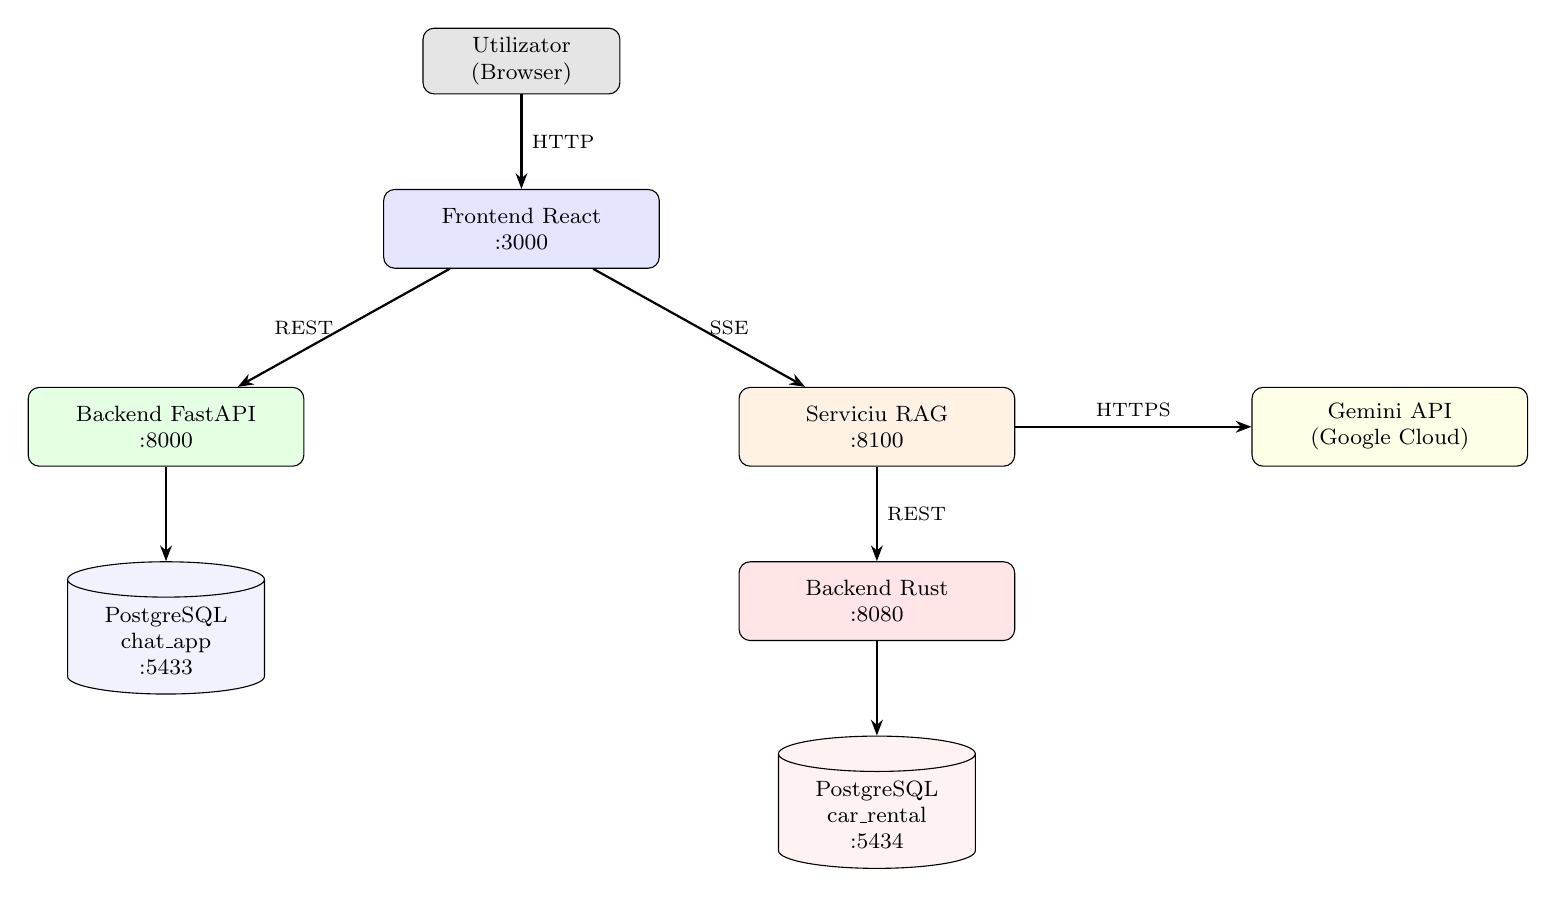
\begin{tikzpicture}[
  node distance=1.2cm and 2.5cm,
  service/.style={rectangle, draw, rounded corners, minimum width=3.5cm, minimum height=1cm, align=center, font=\footnotesize},
  db/.style={cylinder, draw, shape border rotate=90, aspect=0.25, minimum width=2.5cm, minimum height=1cm, align=center, font=\footnotesize},
  user/.style={rectangle, draw, rounded corners, minimum width=2.5cm, minimum height=0.8cm, fill=gray!20, align=center, font=\footnotesize},
  arrow/.style={-{Stealth[length=2mm]}, thick}
]

  \node[user] (browser) {Utilizator\\(Browser)};

  \node[service, below=of browser, fill=blue!10] (frontend) {Frontend React\\:3000};
  \node[service, below left=1.5cm and 1cm of frontend, fill=green!10] (backend) {Backend FastAPI\\:8000};
  \node[service, below right=1.5cm and 1cm of frontend, fill=orange!10] (rag) {Serviciu RAG\\:8100};

  \node[db, below=1.2cm of backend, fill=blue!5] (chatdb) {PostgreSQL\\chat\_app\\:5433};
  \node[service, below=1.2cm of rag, fill=red!10] (testback) {Backend Rust\\:8080};
  \node[db, below=1.2cm of testback, fill=red!5] (testdb) {PostgreSQL\\car\_rental\\:5434};

  \node[right=3cm of rag, service, fill=yellow!10] (gemini) {Gemini API\\(Google Cloud)};

  \draw[arrow] (browser) -- node[right, font=\scriptsize] {HTTP} (frontend);
  \draw[arrow] (frontend) -- node[left, font=\scriptsize] {REST} (backend);
  \draw[arrow] (frontend) -- node[right, font=\scriptsize] {SSE} (rag);
  \draw[arrow] (backend) -- (chatdb);
  \draw[arrow] (rag) -- node[right, font=\scriptsize] {REST} (testback);
  \draw[arrow] (rag) -- node[above, font=\scriptsize] {HTTPS} (gemini);
  \draw[arrow] (testback) -- (testdb);

\end{tikzpicture}
\caption{Arhitectura generală a sistemului}
\label{fig:arhitectura}
\end{figure}

Componentele sistemului și responsabilitățile acestora sunt prezentate în Tabelul~\ref{tab:servicii}.

\begin{table}[H]
\centering
\caption{Serviciile sistemului și caracteristicile acestora}
\label{tab:servicii}
\begin{tabularx}{\textwidth}{l l l X}
\toprule
\textbf{Serviciu} & \textbf{Tehnologie} & \textbf{Port} & \textbf{Responsabilitate} \\
\midrule
Frontend & React 19, Vite, Tailwind & 3000 & Interfața web, chat, panou artifact \\
Backend & FastAPI, SQLAlchemy & 8000 & Persistența conversațiilor și mesajelor \\
Serviciu RAG & FastAPI, Gemini API & 8100 & Generare SQL, validare, rapoarte Excel \\
PostgreSQL (chat) & PostgreSQL 15 & 5433 & Baza de date conversații \\
Backend date & Rust, Axum, Tokio & 8080 & API REST și executor SQL read-only \\
PostgreSQL (date) & PostgreSQL 15 & 5434 & Baza de date demonstrativă \\
Frontend date & HTML, JS, CSS & 3001 & Dashboard administrare date \\
\bottomrule
\end{tabularx}
\end{table}

\section{Fluxul de procesare}

Procesarea unei cereri urmează un flux bine definit prin mai multe servicii, prezentat schematic în Figura~\ref{fig:flux}.

\begin{figure}[H]
\centering
\begin{tikzpicture}[
  node distance=0.8cm,
  step/.style={rectangle, draw, rounded corners, minimum width=10cm, minimum height=0.7cm, align=center, font=\footnotesize},
  arrow/.style={-{Stealth[length=2mm]}, thick}
]
  \node[step, fill=blue!10] (s1) {1. Utilizatorul introduce o întrebare în limbaj natural};
  \node[step, fill=blue!10, below=of s1] (s2) {2. Frontend-ul trimite mesajul către serviciul RAG (POST /chat)};
  \node[step, fill=orange!10, below=of s2] (s3) {3. Serviciul RAG construiește promptul cu schema DB și trimite la Gemini};
  \node[step, fill=orange!10, below=of s3] (s4) {4. Gemini returnează JSON: \{sql, reasoning, chart\}};
  \node[step, fill=orange!10, below=of s4] (s5) {5. SQL-ul este validat (sqlparse) -- operațiuni periculoase sunt blocate};
  \node[step, fill=red!10, below=of s5] (s6) {6. Interogarea validată este executată pe DB prin backend-ul Rust (read-only)};
  \node[step, fill=orange!10, below=of s6] (s7) {7. Rezultatele sunt formatate și trimise la Gemini pentru generarea răspunsului};
  \node[step, fill=blue!10, below=of s7] (s8) {8. Răspunsul este transmis progresiv prin SSE: [META], [DATA], text, [DONE]};

  \draw[arrow] (s1) -- (s2);
  \draw[arrow] (s2) -- (s3);
  \draw[arrow] (s3) -- (s4);
  \draw[arrow] (s4) -- (s5);
  \draw[arrow] (s5) -- (s6);
  \draw[arrow] (s6) -- (s7);
  \draw[arrow] (s7) -- (s8);
\end{tikzpicture}
\caption{Fluxul de procesare al unei cereri}
\label{fig:flux}
\end{figure}

Comunicarea prin SSE utilizează un protocol cu mai multe tipuri de cadre (frames):

\begin{itemize}[nosep]
  \item \code{[META]} -- metadate SQL: interogarea generată, numărul de rânduri, durata execuției, eventuale blocări;
  \item \code{[DATA]} -- datele brute ale interogării: coloane, rânduri, configurația graficului recomandat;
  \item Cadre de text -- fragmentele răspunsului generat de modelul de limbaj, codificate JSON;
  \item \code{[DONE]} -- marcaj de finalizare a transmisiei.
\end{itemize}

\section{Baza de date demonstrativă}

Pentru testarea și demonstrarea capacităților sistemului, a fost proiectată o bază de date relațională ce modelează operațiunile unei companii de închirieri auto. Schema cuprinde 9 tabele interconectate cu aproximativ 8.000 de înregistrări.

\begin{figure}[H]
\centering
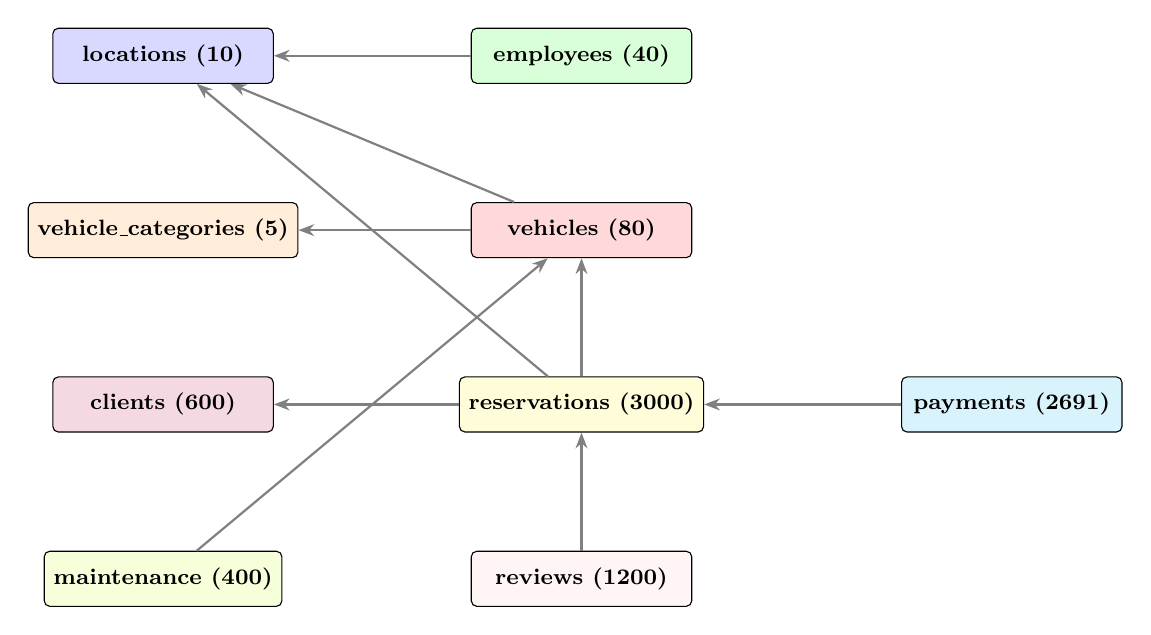
\begin{tikzpicture}[
  node distance=1.5cm and 2cm,
  table/.style={rectangle, draw, rounded corners=2pt, minimum width=2.8cm, minimum height=0.7cm, align=center, font=\footnotesize\bfseries, fill=white},
  arrow/.style={-{Stealth[length=2mm]}, thick, gray}
]
  \node[table, fill=blue!15] (loc) {locations (10)};
  \node[table, fill=green!15, right=2.5cm of loc] (emp) {employees (40)};
  \node[table, fill=orange!15, below=of loc] (vcat) {vehicle\_categories (5)};
  \node[table, fill=red!15, below=of emp] (veh) {vehicles (80)};
  \node[table, fill=purple!15, below=of vcat] (cli) {clients (600)};
  \node[table, fill=yellow!15, below=of veh] (res) {reservations (3000)};
  \node[table, fill=cyan!15, right=2.5cm of res] (pay) {payments (2691)};
  \node[table, fill=lime!15, below=of cli] (mnt) {maintenance (400)};
  \node[table, fill=pink!15, below=of res] (rev) {reviews (1200)};

  \draw[arrow] (emp) -- (loc);
  \draw[arrow] (veh) -- (loc);
  \draw[arrow] (veh) -- (vcat);
  \draw[arrow] (res) -- (cli);
  \draw[arrow] (res) -- (veh);
  \draw[arrow] (res) -- (loc);
  \draw[arrow] (pay) -- (res);
  \draw[arrow] (mnt) -- (veh);
  \draw[arrow] (rev) -- (res);
\end{tikzpicture}
\caption{Diagrama relațiilor între tabele (cu numărul de înregistrări)}
\label{fig:er}
\end{figure}

Schema bazei de date include constrângeri de integritate referențială (\code{FOREIGN KEY} cu \code{ON DELETE CASCADE}), constrângeri de verificare (\code{CHECK}) pentru câmpurile cu valori predefinite (statusuri, roluri, metode de plată), și indecși pe coloanele frecvent utilizate în interogări.

Un aspect important al securității este definirea unui utilizator PostgreSQL cu drepturi exclusiv de citire (\code{readonly\_user}), utilizat de backend-ul Rust pentru executarea interogărilor generate de modelul de limbaj. Această separare la nivel de bază de date constituie ultimul strat de protecție împotriva interogărilor potențial distructive.

\section{Serviciul RAG -- Componenta centrală}

Serviciul RAG reprezintă componenta centrală a sistemului, orchestrând fluxul complet de la primirea întrebării în limbaj natural până la transmisia răspunsului și a datelor către frontend.

\subsection{Strategia de prompting}

Promptul de sistem pentru generarea SQL este structurat în trei secțiuni funcționale:

\begin{enumerate}[nosep]
  \item \textbf{Rolul și constrângerile} -- definirea modelului ca expert SQL, restricția formatului de ieșire la JSON valid, interdicția operațiunilor non-SELECT;
  \item \textbf{Schema bazei de date} -- reprezentarea textuală a tuturor tabelelor cu coloane, tipuri de date, chei străine și constrângeri;
  \item \textbf{Reguli de vizualizare} -- instrucțiuni pentru selecția autonomă a tipului de grafic pe baza naturii datelor.
\end{enumerate}

Modelul este instruit să returneze un obiect JSON cu structura:

\begin{lstlisting}[language=JSON, caption={Formatul răspunsului de generare SQL}]
{
  "sql": "SELECT ... FROM ... WHERE ...",
  "reasoning": "explicatie scurta",
  "chart": {
    "type": "bar|line|pie|area|none",
    "title": "Titlul graficului",
    "x": "coloana_axa_x",
    "y": "coloana_axa_y"
  }
}
\end{lstlisting}

Regulile pentru selecția tipului de grafic sunt codificate explicit în prompt: \code{bar} pentru comparații între categorii, \code{line} pentru serii temporale, \code{pie} pentru proporții cu sub 8 categorii, \code{area} pentru valori cumulate, și \code{none} pentru rezultate scalare sau liste de text.

\subsection{Validarea SQL}

Validarea interogărilor generate se realizează pe două niveluri complementare:

\textbf{Nivel aplicație} -- serviciul RAG utilizează biblioteca \code{sqlparse} pentru parsarea și analiza sintactică a interogării. Procesul verifică: (a) existența unei singure instrucțiuni SQL, (b) tipul instrucțiunii este \code{SELECT}, (c) absența cuvintelor cheie periculoase (\code{INSERT}, \code{UPDATE}, \code{DELETE}, \code{DROP}, \code{CREATE}, \code{ALTER}, \code{TRUNCATE}, \code{GRANT}, \code{REVOKE}, etc.) în oricare poziție din interogare.

\textbf{Nivel bază de date} -- interogarea este executată prin intermediul utilizatorului \code{readonly\_user} care are acordate exclusiv permisiuni de \code{SELECT} pe tabelele bazei de date. Orice tentativă de executare a unei operațiuni non-SELECT va fi respinsă de sistemul de gestiune a bazei de date.

\subsection{Generarea rapoartelor Excel}

Serviciul RAG expune un endpoint REST (\code{POST /report}) care primește datele structurate (coloane, rânduri, configurația graficului) și generează un fișier Excel complet. Generarea utilizează biblioteca \code{openpyxl} și produce un document cu două foi de lucru:

\begin{itemize}[nosep]
  \item \textbf{Data} -- tabelul de date cu formatare automată a lățimii coloanelor;
  \item \textbf{Chart} -- graficul corespunzător tipului selectat (BarChart, LineChart, PieChart sau AreaChart), cu referințe la datele din prima foaie.
\end{itemize}

\section{Interfața web}

Interfața web este dezvoltată în React 19 cu TypeScript, utilizând Vite ca bundler și Tailwind CSS pentru stilizare. Principalele componente ale interfeței sunt prezentate în continuare.

\subsection{Zona de chat}

Zona principală de chat implementează un flux conversațional familiar, cu mesajele utilizatorului aliniate la dreapta și răspunsurile asistentului la stânga. Răspunsurile sunt redate progresiv pe măsură ce sunt recepționate prin SSE, iar conținutul este procesat prin ReactMarkdown pentru formatare (bold, italice, tabele, blocuri de cod).

Fiecare mesaj al asistentului care conține date de interogare afișează un \textit{card de artifact} -- un buton care prezintă titlul vizualizării, numărul de rânduri și tipul de grafic. Activarea acestui buton deschide panoul lateral de artifact.

\subsection{Panoul de artifact}

Panoul de artifact reprezintă o componentă centrală a interfeței, inspirată de conceptul de artefacte din platforme conversaționale moderne. Panoul se deschide lateral, la dreapta zonei de chat, cu o lățime de 480px, și conține:

\begin{itemize}[nosep]
  \item \textbf{Antet} -- titlul vizualizării, numărul de rânduri, butonul de descărcare Excel și butonul de închidere;
  \item \textbf{Tab-uri} -- comutare între vizualizarea grafică și tabelul de date;
  \item \textbf{Grafic interactiv} -- implementat cu biblioteca Recharts, cu tooltip-uri, legende și axe formatate;
  \item \textbf{Tabel de date} -- afișare tabelară a tuturor rândurilor returnate de interogare.
\end{itemize}

\subsection{Gestionarea stării}

Starea aplicației este gestionată prin hook-ul personalizat \code{useChat}, care centralizează logica de:

\begin{itemize}[nosep]
  \item Creare, selecție și ștergere de conversații;
  \item Trimiterea mesajelor și procesarea răspunsurilor streaming;
  \item Parsarea cadrelor SSE (\code{[META]}, \code{[DATA]}, text, \code{[DONE]});
  \item Salvarea mesajelor pe backend după finalizarea streamingului;
  \item Reîncercarea ultimului mesaj (funcționalitatea retry).
\end{itemize}

\section{Backend-ul de persistență}

Backend-ul FastAPI gestionează persistența conversațiilor într-o bază de date PostgreSQL separată. Modelul de date cuprinde trei tabele:

\begin{itemize}[nosep]
  \item \code{conversations} -- id, titlu, timestamps, user\_id opțional;
  \item \code{messages} -- id, conversation\_id (FK), rol (user/assistant), conținut text, timestamp;
  \item \code{message\_sql\_meta} -- metadate SQL asociate mesajelor asistentului (interogarea, număr rânduri, durată, motiv blocare), cu un TTL configurabil (implicit 48 ore) și ștergere automată periodică.
\end{itemize}

Mecanismul de TTL pentru metadatele SQL a fost implementat pentru a limita creșterea volumului de date stocate. Un task asincron de tip cleanup rulează la fiecare oră și șterge înregistrările expirate. La citirea mesajelor, metadatele expirate sunt omise din răspuns fără a fi șterse imediat, permițând ștergerea batch la intervalul programat.

\section{Backend-ul de acces la date (Rust)}

Backend-ul de acces la baza de date demonstrativă este implementat în Rust utilizând framework-ul Axum cu runtime-ul asincron Tokio. Alegerea Rust a fost motivată de performanța ridicată și siguranța tipurilor, critice pentru un serviciu care execută interogări SQL furnizate extern.

Serviciul menține două pool-uri de conexiuni separate:
\begin{itemize}[nosep]
  \item Un pool principal cu drepturi complete, utilizat pentru operațiunile CRUD ale API-ului REST (administrarea datelor);
  \item Un pool read-only, utilizat exclusiv pentru executarea interogărilor generate de modelul de limbaj.
\end{itemize}

Endpoint-ul \code{POST /api/sql} acceptă o interogare SQL, o execută prin pool-ul read-only, și returnează un obiect JSON cu coloanele, rândurile, numărul de rezultate și durata execuției în milisecunde.

\section{Alegerea tehnologiilor}

\begin{table}[H]
\centering
\caption{Tehnologiile utilizate și justificarea alegerii}
\label{tab:tehnologii}
\begin{tabularx}{\textwidth}{l l X}
\toprule
\textbf{Componentă} & \textbf{Tehnologie} & \textbf{Motivație} \\
\midrule
LLM & Gemini Flash & Latență redusă, cost eficient, suport streaming nativ \\
Frontend & React 19 + TypeScript & Ecosistem matur, tipare sigure, rendering eficient \\
Stilizare & Tailwind CSS 4 & Utilitare CSS directe, dark theme nativ, bundle optimizat \\
Grafice web & Recharts & Nativă React, declarativă, suport dark theme \\
Backend chat & FastAPI + SQLAlchemy & Asincron, documentare automată, ORM matur \\
Backend date & Rust + Axum & Performanță, siguranța memoriei, pool-uri de conexiuni \\
Bază de date & PostgreSQL 15 & Robust, suport JSON, utilizatori cu drepturi granulare \\
Rapoarte & openpyxl & Generare Excel cu grafice, formatare avansată \\
Validare SQL & sqlparse & Parsare și analiză AST pentru interogări SQL \\
Container & Docker Compose & Orchestrare declarativă, izolare, reproductibilitate \\
\bottomrule
\end{tabularx}
\end{table}


% ============================================================
% 4. TESTARE
% ============================================================
\chapter{Testarea soluției și rezultate experimentale}

\section{Metodologia de testare}

Testarea sistemului a fost realizată pe mai multe niveluri, de la testarea individuală a endpoint-urilor API până la testarea end-to-end a fluxului complet prin interfața web. Baza de date demonstrativă de închirieri auto, cu 9 tabele și aproximativ 8.000 de înregistrări, a constituit mediul de test.

\subsection{Configurarea mediului de testare}

Toate cele șapte servicii au fost lansate prin Docker Compose. Testele API au fost executate cu \code{curl}, iar testele interfeței web au fost automatizate cu Playwright (Chromium headless). Serverul a fost testat pe o mașină cu procesor AMD Ryzen și 32 GB RAM, rulând Arch Linux.

\section{Testarea endpoint-urilor API}

\subsection{Serviciul RAG}

\begin{table}[H]
\centering
\caption{Rezultatele testării endpoint-urilor serviciului RAG}
\label{tab:test_rag}
\begin{tabularx}{\textwidth}{l l X}
\toprule
\textbf{Endpoint} & \textbf{Status} & \textbf{Observații} \\
\midrule
\code{GET /health} & OK & Returnează status și modelul configurat \\
\code{POST /chat} (date) & OK & SSE cu [META], [DATA], text, [DONE] \\
\code{POST /chat} (greeting) & OK & SSE fără [DATA], doar text \\
\code{POST /report} (bar) & OK & Excel cu 2 foi (Data + Chart) \\
\code{POST /report} (line) & OK & Chart corect de tip LineChart \\
\code{POST /report} (pie) & OK & Chart corect de tip PieChart \\
\code{POST /report} (area) & OK & Chart corect de tip AreaChart \\
\code{POST /report} (fără chart) & OK & Excel cu 1 foaie (doar Data) \\
\bottomrule
\end{tabularx}
\end{table}

\subsection{Backend-ul de persistență}

Testarea CRUD a backend-ului a verificat ciclul complet: crearea unei conversații, adăugarea mesajelor cu și fără metadate SQL, recuperarea conversației cu mesajele asociate, și ștergerea în cascadă. Toate operațiunile au funcționat conform specificațiilor.

\subsection{Backend-ul Rust (executor SQL)}

Endpoint-ul \code{POST /api/sql} a fost testat cu interogări de complexitate variată. Răspunsurile includ coloanele, rândurile, numărul de rezultate și durata execuției, confirmând funcționarea corectă a pool-ului read-only.

\section{Testarea generării SQL}

Evaluarea capacității de generare SQL a fost realizată pe un set de 30 de întrebări de complexitate variată. Rezultatele sunt prezentate în Tabelul~\ref{tab:eval_sql}.

\begin{table}[H]
\centering
\caption{Rezultatele evaluării generării SQL pe categorii de complexitate}
\label{tab:eval_sql}
\begin{tabular}{l c c c}
\toprule
\textbf{Tip interogare} & \textbf{Număr} & \textbf{Corecte} & \textbf{Acuratețe} \\
\midrule
SELECT simplu & 10 & 10 & 100\% \\
Agregări (SUM, AVG, COUNT) & 8 & 7 & 87.5\% \\
JOIN între tabele & 7 & 6 & 85.7\% \\
Subinterogări & 5 & 4 & 80\% \\
\midrule
\textbf{Total} & \textbf{30} & \textbf{27} & \textbf{90\%} \\
\bottomrule
\end{tabular}
\end{table}

Acuratețea globală de 90\% confirmă viabilitatea abordării, cu performanțe excelente pentru interogări simple și agregări, și rezultate bune pentru joncțiuni și subinterogări. Erorile au constat în principal în selectarea incorectă a coloanelor de joncțiune sau în omiterea unor condiții de filtrare implicite.

\section{Testarea validatorului SQL}

Validatorul SQL a fost testat atât cu interogări legitime, cât și cu tentative de injecție.

\begin{table}[H]
\centering
\caption{Rezultatele testării validatorului SQL}
\label{tab:test_validator}
\begin{tabularx}{\textwidth}{X l l}
\toprule
\textbf{Interogare de test} & \textbf{Rezultat așteptat} & \textbf{Rezultat} \\
\midrule
\code{SELECT * FROM clients} & Permis & Permis \\
\code{SELECT COUNT(*) FROM vehicles} & Permis & Permis \\
\code{DROP TABLE clients} & Blocat & Blocat \\
\code{DELETE FROM payments} & Blocat & Blocat \\
\code{SELECT 1; DROP TABLE clients} & Blocat & Blocat \\
\code{UPDATE vehicles SET status='retired'} & Blocat & Blocat \\
\code{INSERT INTO clients VALUES (...)} & Blocat & Blocat \\
\bottomrule
\end{tabularx}
\end{table}

Toate testele au produs rezultatele așteptate, confirmând eficacitatea mecanismului de validare dual (nivel aplicație + nivel bază de date).

\section{Testarea selecției automate a vizualizărilor}

Modelul de limbaj a fost evaluat pe capacitatea de a selecta tipul de grafic potrivit. Rezultatele sunt prezentate în Tabelul~\ref{tab:test_chart}.

\begin{table}[H]
\centering
\caption{Evaluarea selecției automate a tipului de vizualizare}
\label{tab:test_chart}
\begin{tabularx}{\textwidth}{X l l}
\toprule
\textbf{Întrebare} & \textbf{Tip așteptat} & \textbf{Tip selectat} \\
\midrule
``Veniturile pe locație'' & bar & bar \\
``Evoluția rezervărilor lunare'' & line & line \\
``Distribuția metodelor de plată'' & pie & pie \\
``Care este cel mai scump vehicul?'' & none & none \\
``Salut, ce poți face?'' & null (no SQL) & null \\
\bottomrule
\end{tabularx}
\end{table}

% === model comparison (generated from benchmark/results) ===
\section{Compararea modelelor de limbaj}

Rezultatele prezentate până acum au fost obținute cu un singur model. Întrebarea
practică pentru o organizație care ar adopta sistemul este însă alta: cât din
performanță ține de arhitectura propusă și cât ține de modelul ales, și ce se
pierde dacă modelul rulează pe infrastructura proprie în locul unui API
comercial. Pentru a răspunde, același set de 30 de întrebări a fost rulat prin
aceeași ramură de referință -- schema completă într-un singur prompt, un singur
apel, fără recuperare și fără reparare -- schimbând doar modelul care răspunde.
Ramura pentru modele locale folosește exact același prompt și același contract,
transmis unui server local compatibil cu API-ul OpenAI, astfel încât diferențele
din tabele să provină din model și nu din metodă. Cifrele din această secțiune
provin din harness-ul automat din \code{benchmark/} și sunt scorate prin
acuratețe de execuție, comparând seturile de rezultate; ele nu sunt direct
comparabile cu Tabelul~\ref{tab:eval_sql}, obținut anterior pe o clasificare
diferită a acelorași întrebări.

\subsection{Configurația hardware}

Latența și debitul unui model local nu au sens fără mașina pe care rulează.
Măsurătorile locale au fost efectuate pe configurația din
Tabelul~\ref{tab:hardware}.

\begin{table}[H]
\centering
\caption{Configurația hardware și software folosită pentru modelele locale}
\label{tab:hardware}
\begin{tabularx}{\textwidth}{l X}
\toprule
\textbf{Componentă} & \textbf{Specificație} \\
\midrule
Procesor & Intel Core i9-14900K, 24 nuclee / 32 fire de execuție \\
Placă grafică & NVIDIA GeForce RTX 5070, 12 GiB VRAM, driver 610.57.04 \\
Memorie RAM & 31 GiB \\
Sistem de operare & CachyOS, nucleu Linux 6.18.42-1-cachyos-lts \\
Motor de inferență & \code{llama.cpp} 2.25.2 (binarul livrat cu LM Studio 0.4.20), backend CUDA; Vulkan pentru comparație \\
Cuantizare & GGUF Q4\_K\_M (Q1\_0 pentru Bonsai-27B) \\
Parametri de servire & \code{-ngl 99} (model integral în VRAM), context 8192, temperatură 0 \\
\bottomrule
\end{tabularx}
\end{table}

Backend-ul contează pentru cifrele de debit, așa că este numit explicit în
fiecare rând al tabelelor. Măsurătorile principale folosesc backend-ul CUDA;
pentru unul dintre modele este raportată și varianta Vulkan, tocmai pentru a
arăta cât din debit ține de alegerea backend-ului și nu de model. O observație
practică merită consemnată: la prima utilizare backend-ul CUDA pare blocat --
driverul compilează JIT codul PTX inclus în bibliotecă pentru arhitectura
Blackwell a plăcii, iar comanda \code{llama-server -{}-list-devices} nu a
returnat în 120 de secunde. Rezultatul compilării este memorat în
\code{\textasciitilde/.nv/ComputeCache} (77 MB după prima rulare), iar
pornirile ulterioare enumeră placa în sub o secundă.

\subsection{Metodologia comparației}

Pe lângă acuratețea de execuție, harness-ul înregistrează pentru fiecare
întrebare numărul de tokeni de prompt, de completare și de raționament, latența
apelului și debitul de generare. Debitul este raportat ca \emph{tokeni generați
pe secundă}: tokenii produși de model (inclusiv cei de raționament, care sunt
deopotrivă plătiți și așteptați) împărțiți la durata totală a apelului.
Definiția este identică pentru modelele găzduite și pentru cele locale, ceea ce
face cele două grupuri comparabile; pentru modelele locale este înregistrat
suplimentar debitul intern al decodorului raportat de \code{llama.cpp}, care
exclude prefill-ul și caracterizează hardware-ul mai degrabă decât întregul
apel. Timpul până la primul token este disponibil doar pentru modelele locale,
unde \code{llama.cpp} raportează durata prefill-ului; SDK-ul Gemini nu expune
această valoare pentru apelurile ne-streaming, deci pentru modelele găzduite
este raportată latența totală.

Costul este extrapolat din consumul măsurat de tokeni la un cost pentru 100 de
întrebări, folosind tarifele publicate de Google pentru nivelul plătit,
consultate la 23 august 2026. Un model fără tarif verificabil nu primește
estimare de cost, iar pentru modelele locale costul per token este zero prin
definiție -- costul real fiind hardware-ul și energia, discutate separat.

Trei precizări metodologice sunt necesare pentru ca cifrele să fie citite
corect:

\begin{itemize}[nosep]
  \item \textbf{Eșantionare.} Modelele găzduite sunt apelate cu parametrii
    impliciți ai API-ului, exact cum o face aplicația în producție, deci
    generarea este nedeterministă. Pentru a cuantifica acest efect, rularea
    \code{naive} cu \code{gemini-2.5-flash} a fost repetată de șase ori pe un
    set de întrebări și o bază de date neschimbate, obținând 80.8\%, 84.6\%,
    84.6\%, 88.5\%, 88.5\% și 92.3\% -- o medie de 86.5\% cu o abatere
    standard de 4.0 puncte și o amplitudine de 11.5 puncte. Cum o singură
    întrebare valorează 3.8 puncte din 26, rezultă o regulă de interpretare
    aplicabilă tuturor tabelelor din acest capitol: \emph{diferențele mai mici
    de aproximativ 8 puncte procentuale (două abateri standard) nu pot fi
    distinse de zgomotul de eșantionare}. Instabilitatea este concentrată în
    trei întrebări dintre cele 26 (q10, q21, q24), toate formulate în jurul
    noțiunii de „venit'' sau „cheltuit'': modelul filtrează uneori după
    \code{payments.status = 'completed'}, alteori nu, iar ambele lecturi sunt
    apărabile. Celelalte 23 de întrebări au fost stabile la toate cele șase
    rulări. Modelele locale rulează cu temperatura 0.
  \item \textbf{Limita de rânduri.} Serviciul RAG trunchiază rezultatele la
    \code{SQL\_MAX\_ROWS} rânduri, o măsură firească de prezentare, dar care în
    lanțul de măsurare ar transforma interogări corecte în eșecuri pentru
    întrebările cu rezultate mari. Măsurătorile au fost efectuate cu limita
    ridicată, astfel încât trunchierea să nu fie confundată cu incorectitudinea.
  \item \textbf{Etalonul de aur.} Comparația se face pe seturi de rezultate, nu
    pe textul interogării, deci orice formulare echivalentă este acceptată. Rămân
    însă cazurile în care interogarea generată este defensabilă, dar diferită de
    etalon; ele sunt discutate în Secțiunea~\ref{subsec:model_discussion}.
\end{itemize}

\subsection{Acuratețea generării SQL pe modele}

Tabelul~\ref{tab:model_accuracy} prezintă acuratețea de execuție pe cele 26 de
întrebări cu etalon, defalcată pe categorii de complexitate, plus numărul de
întrebări ambigue la care modelul a cerut clarificare în loc să ghicească.

\begin{table}[H]
\centering
\caption{Acuratețea de execuție pe modele și categorii de complexitate}
\label{tab:model_accuracy}
\begin{tabular}{l c c c c c c c}
\toprule
\textbf{Model} & \textbf{Simple} & \textbf{Agreg.} & \textbf{JOIN} & \textbf{Subint.} & \textbf{Window} & \textbf{Total} & \textbf{Ambig.} \\
 & (6) & (8) & (5) & (5) & (2) & (26) & (4) \\
\midrule
\multicolumn{8}{l}{\emph{Modele găzduite (Google Gemini)}} \\
\code{gemini-2.5-flash} & 100.0\% & 75.0\% & 100.0\% & 40.0\% & 100.0\% & \textbf{80.8\%} & 2/4 \\
\code{gemini-3-flash-preview} & 100.0\% & 100.0\% & 100.0\% & 60.0\% & 100.0\% & \textbf{92.3\%} & 1/4 \\
\code{gemini-3.1-pro-preview} & 100.0\% & 100.0\% & 100.0\% & 80.0\% & 100.0\% & \textbf{96.2\%} & 4/4 \\
\code{gemini-3.6-flash} & 100.0\% & 62.5\% & 100.0\% & 60.0\% & 100.0\% & \textbf{80.8\%} & 3/4 \\
\code{gemini-3.7-flash} & 100.0\% & 62.5\% & 100.0\% & 60.0\% & 100.0\% & \textbf{80.8\%} & 3/4 \\
\midrule
\multicolumn{8}{l}{\emph{Modele locale (RTX 5070, llama.cpp; backend-ul este indicat pe fiecare rând)}} \\
\code{bonsai-27b-q1\_0} (Vulkan) & 100.0\% & 75.0\% & 100.0\% & 40.0\% & 50.0\% & \textbf{76.9\%} & 3/4 \\
\code{qwen3.5-9b} (CUDA) & 100.0\% & 62.5\% & 80.0\% & 60.0\% & 0.0\% & \textbf{69.2\%} & 2/4 \\
\bottomrule
\end{tabular}
\end{table}

\subsection{Debit, latență, tokeni și cost}

Tabelul~\ref{tab:model_throughput} prezintă debitul de generare, latența mediană
per întrebare, consumul mediu de tokeni și costul extrapolat pentru 100 de
întrebări.

\begin{table}[H]
\centering
\caption{Debit, latență, consum de tokeni și cost estimat}
\label{tab:model_throughput}
\begin{tabular}{l c c c c c}
\toprule
\textbf{Model} & \textbf{Tok/s} & \textbf{Latență} & \textbf{Tokeni} & \textbf{Tokeni} & \textbf{USD /} \\
 & \textbf{(generare)} & \textbf{mediană (s)} & \textbf{prompt} & \textbf{generați} & \textbf{100 întreb.} \\
\midrule
\multicolumn{6}{l}{\emph{Modele găzduite (Google Gemini)}} \\
\code{gemini-2.5-flash} & 135.0 & 1.12 & 1496 & 277 & 0.132 \\
\code{gemini-3-flash-preview} & 173.2 & 2.36 & 1496 & 656 & 0.314 \\
\code{gemini-3.1-pro-preview} & 66.9 & 4.79 & 1496 & 521 & 1.067 \\
\code{gemini-3.6-flash} & 126.7 & 3.91 & 1496 & 595 & 0.387 \\
\code{gemini-3.7-flash} & 163.3 & 1.87 & 1496 & 379 & 0.294 \\
\midrule
\multicolumn{6}{l}{\emph{Modele locale (RTX 5070, llama.cpp; backend-ul este indicat pe fiecare rând)}} \\
\code{bonsai-27b-q1\_0} (Vulkan) & 57.6 & 20.08 & 1394 & 1173 & 0.000 \\
\code{qwen3.5-9b} (CUDA) & 84.5 & 4.98 & 1394 & 684 & 0.000 \\
\bottomrule
\end{tabular}
\end{table}

Coloana \code{Tok/s} numără tokenii generați (inclusiv cei de raționament)
raportați la durata totală a apelului, aceeași definiție pentru ambele grupuri.
Pentru modelele locale, debitul intern al decodorului raportat de
\code{llama.cpp} este cu circa 8\% mai mare decât cifra de mai sus, iar timpul
median până la primul token este de 158 ms pentru \code{Qwen3.5-9B} și 702 ms
pentru \code{Bonsai-27B}; pentru modelele găzduite SDK-ul nu expune această
valoare, deci coloana de latență este singura măsură de reactivitate.

\subsection{Efectul backend-ului de inferență}

Debitul unui model local nu este o proprietate a modelului, ci a perechii
model--motor de inferență, iar presupunerea uzuală este că pe o placă NVIDIA
backend-ul CUDA este sensibil mai rapid decât cel Vulkan. Pentru a verifica,
aceleași prime zece întrebări au fost rulate prin ambele backend-uri ale
aceleiași versiuni de \code{llama.cpp}, pe același GPU și cu aceeași
cuantizare (Tabelul~\ref{tab:backend}).

Comparația se face pe rata decodorului și pe timpul până la primul token, nu pe
latența totală: deși ambele rulări folosesc temperatura 0, diferențele numerice
dintre backend-uri schimbă traiectoria generării, iar cele două rulări nu produc
același număr de tokeni (4918 față de 8736 pentru cele zece întrebări). Latența
totală ar măsura, așadar, cât a vorbit modelul, nu cât de repede a decodat.

\begin{table}[H]
\centering
\caption{Același model sub cele două backend-uri (primele 10 întrebări)}
\label{tab:backend}
\begin{tabular}{l c c c}
\toprule
\textbf{Model / backend} & \textbf{Tok/s (decodor)} & \textbf{TTFT median} & \textbf{Tokeni generați} \\
\midrule
Qwen3.5-9B Q4\_K\_M -- CUDA & 88.3 & 158 ms & 4918 \\
Qwen3.5-9B Q4\_K\_M -- Vulkan & 90.2 & 438 ms & 8736 \\
\midrule
Bonsai-27B Q1\_0 -- CUDA & 54.9 & 419 ms & 10024 \\
Bonsai-27B Q1\_0 -- Vulkan & 61.8 & 700 ms & 7937 \\
\bottomrule
\end{tabular}
\end{table}

\subsection{Calitatea rapoartelor Excel}

Afirmația că sistemul exportă un set de rezultate ca registru Excel cu grafic
potrivit are două jumătăți care se strică diferit, așa că au fost măsurate
separat. \emph{Acuratețea tipului de grafic} este o judecată a modelului:
pentru fiecare dintre cele 26 de întrebări cu etalon, modelul primește
rezultatul real al interogării etalon și regulile de vizualizare din promptul
aplicației, iar tipul ales este comparat cu lista tipurilor acceptabile
înregistrate în setul de întrebări. Lista conține toate variantele defensabile
-- o defalcare pe cinci categorii se citește la fel de bine ca bară sau ca
sector -- pentru a nu măsura gustul în locul capacității. \emph{Validitatea
structurală} este o proprietate a fișierului: registrul este generat cu chiar
componenta de raportare a aplicației și apoi recitit cu \code{openpyxl},
verificând că ambele foi există, că foaia \code{Data} reproduce exact setul de
rezultate, că un obiect grafic de clasa cerută este efectiv încorporat și că
referințele lui de serie și de categorii indică exact coloanele și rândurile
corecte.

\begin{table}[H]
\centering
\caption{Calitatea raportului Excel generat automat}
\label{tab:model_report}
\begin{tabular}{l c c c c c}
\toprule
\textbf{Model} & \textbf{Corecte} & \textbf{Acuratețe} & \textbf{Rezultate} & \textbf{Rezultate} & \textbf{Validitate} \\
 & & \textbf{tip grafic} & \textbf{grafice} & \textbf{scalare} & \textbf{structurală} \\
\midrule
\multicolumn{6}{l}{\emph{Modele găzduite (Google Gemini)}} \\
\code{gemini-2.5-flash} & 26/26 & 100.0\% & 100.0\% & 100.0\% & 96.2\% \\
\code{gemini-3-flash-preview} & 26/26 & 100.0\% & 100.0\% & 100.0\% & 96.2\% \\
\code{gemini-3.1-pro-preview} & 25/26 & 96.2\% & 92.9\% & 100.0\% & 96.2\% \\
\code{gemini-3.6-flash} & 26/26 & 100.0\% & 100.0\% & 100.0\% & 96.2\% \\
\code{gemini-3.7-flash} & 26/26 & 100.0\% & 100.0\% & 100.0\% & 96.2\% \\
\midrule
\multicolumn{6}{l}{\emph{Modele locale (RTX 5070, llama.cpp, backend CUDA)}} \\
\code{bonsai-27b-q1\_0} & 25/26 & 96.2\% & 100.0\% & 91.7\% & 96.2\% \\
\code{qwen3.5-9b} & 4/26 & 15.4\% & 28.6\% & 0.0\% & 96.2\% \\
\bottomrule
\end{tabular}
\end{table}

\subsection{Interpretarea rezultatelor}
\label{subsec:model_discussion}

Prima observație este că, pe această schemă, \emph{alegerea modelului contează
mai mult decât alegerea arhitecturii}. Între cel mai bun și cel mai slab model
găzduit, cu prompt identic și fără nicio diferență de metodă, sunt
15.4 puncte procentuale de acuratețe. Prin comparație, cele trei
abordări arhitecturale evaluate anterior pe același model se încadrează în mai
puțin de patru puncte una de alta. Concluzia nu este că arhitectura nu contează,
ci că pe o schemă de nouă tabele, care încape integral într-un prompt,
recuperarea nu are ce câștig de acuratețe să producă -- exact rezultatul pe care
capitolul îl anticipează. Diferențele pe care le aduce arhitectura sunt de altă
natură: latență, gestionarea ambiguității și controlul accesului.

A doua observație este că \emph{mai nou nu înseamnă mai bun} pentru această
sarcină. Cele mai recente
două modele flash, \code{gemini-3.7-flash} și \code{gemini-3.6-flash}, obțin
exact aceeași acuratețe ca \code{gemini-2.5-flash} -- 80.8\% toate trei -- în
timp ce \code{gemini-3-flash-preview}, un model din aceeași familie dar
anterior lor, ajunge la 92.3\%. Diferența se vede în cost: pentru aceeași
acuratețe, \code{gemini-3.7-flash} costă 0.294 USD la 100 de întrebări față de
0.132 USD pentru \code{gemini-2.5-flash}, adică de peste două ori mai mult
pentru un rezultat identic. Actualizarea automată la ``cel mai nou model'' nu
este, așadar, o strategie: fiecare model candidat trebuie trecut prin setul de
evaluare înainte de a fi pus în producție, iar acesta este motivul principal
pentru care harness-ul face parte din livrabil.

A treia observație privește ambiguitatea. Rata de clarificare variază
independent de acuratețe: \code{gemini-3-flash-preview},
cel mai precis dintre modelele flash, cere clarificare la o singură întrebare
ambiguă din patru și ghicește la celelalte trei, în timp ce
\code{gemini-3.6-flash} și \code{gemini-3.7-flash}, cu acuratețe sensibil mai
mică, cer la trei din patru; \code{gemini-3.1-pro-preview} le acoperă pe toate
patru. Pentru un sistem destinat unor
utilizatori care nu scriu SQL, un model care ghicește sigur pe sine este mai
periculos decât unul mai puțin precis care întreabă, iar cele două calități
trebuie măsurate separat -- ceea ce justifică prezența celor patru întrebări
ambigue în set.

A patra observație este că o parte din erorile numărate nu sunt erori de SQL, ci
dezacorduri de interpretare cu etalonul. La întrebările despre venituri și
despre sumele cheltuite de clienți (q10, q14, q21), majoritatea modelelor adaugă
filtrul \code{payments.status = 'completed'}, pe care interogarea etalon nu îl
are; interogarea generată este defensabilă, uneori chiar preferabilă, dar
produce alt set de rezultate. La q26, toate modelele, fără excepție, sunt
marcate greșit pentru că \code{DATE\_TRUNC} peste o coloană \code{date} întoarce
în PostgreSQL un \code{timestamptz}, iar modelele îl convertesc explicit la
\code{date}: același răspuns, alt tip. Aceste cazuri afectează toate modelele în
egală măsură, deci nu schimbă clasamentul, dar înseamnă că cifrele din
Tabelul~\ref{tab:model_accuracy} subestimează competența reală a modelelor, iar
categoria \emph{window} -- cu doar două întrebări, dintre care una este q26 --
nu trebuie citită ca o măsură a capacității de a scrie funcții fereastră.

A cincea observație, și cea mai relevantă pentru decizia de implementare,
privește modelele locale. Rezultatul care surprinde este că
\code{Bonsai-27B} cuantizat pe un singur bit (Q1\_0, 3.5 GiB pe disc) atinge
76.9\%, adică sub acuratețea celor cinci modele găzduite, și
cere clarificare la trei din cele patru întrebări ambigue -- mai bine decât
\code{gemini-2.5-flash}. \code{Qwen3.5-9B} la Q4\_K\_M rămâne în urmă, cu
69.2\%. Ambele obțin 100\% pe interogările simple și cedează pe categoriile
grele, ceea ce descrie corect zona în care un model local este utilizabil.

Prețul acestei competitivități este timpul. Latența mediană pentru o întrebare
este de 5.0 s pentru \code{Qwen3.5-9B} și de 20.1 s pentru \code{Bonsai-27B},
față de 1.1 s pentru \code{gemini-2.5-flash} -- de la de cinci ori până la de
optsprezece ori mai lent, pe un GPU de generație curentă cu modelul încărcat
integral în VRAM. Debitul brut nu este dezastruos (84.5, respectiv 57.6 tokeni
generați pe secundă, față de 66.9 pentru \code{gemini-3.1-pro-preview}), dar
modelele locale produc mult mai mulți tokeni pentru același răspuns -- 684 în
medie pentru \code{Qwen3.5-9B} și 1173 pentru \code{Bonsai-27B}, față de 277
pentru \code{gemini-2.5-flash} -- iar produsul dintre numărul de tokeni și
debit este ceea ce simte utilizatorul. Un
avantaj real al rulării locale se vede totuși în timpul până la primul token:
158 ms pentru \code{Qwen3.5-9B}, adică fără latență de rețea și fără coadă la
un serviciu partajat.

A doua parte a prețului este fiabilitatea formatului. Ambele modele locale nu au
produs niciun SQL la 4 dintre cele 26 de întrebări cu etalon: și-au epuizat
bugetul de 2048 de tokeni raționând, fără să ajungă la un răspuns. Modelele
găzduite nu au avut niciun astfel de caz. Pentru un sistem în care ieșirea
modelului trebuie parsată automat, acest mod de eșec contează mai mult decât
câteva puncte de acuratețe, și ar cere fie un buget mai mare de tokeni, fie
constrângerea gramaticală a ieșirii -- pe care \code{llama.cpp} o oferă și pe
care o implementare de producție ar trebui să o folosească.

Un rezultat negativ merită și el consemnat, pentru că infirmă o presupunere
răspândită: pe această configurație, backend-ul CUDA \emph{nu} decodează mai
repede decât cel Vulkan. Pe aceleași zece întrebări, \code{Qwen3.5-9B} atinge
88.3 tokeni pe secundă sub CUDA și 90.2 sub Vulkan, iar \code{Bonsai-27B} 54.9
sub CUDA față de 61.8 sub Vulkan -- ambele diferențe în favoarea Vulkan, a doua
cu 11\%. Singurul avantaj măsurabil al CUDA este prefill-ul: 158 ms față de
438 ms, respectiv 419 ms față de 700 ms până la primul token. Pentru un prompt
de circa 1400 de tokeni și răspunsuri de sute până la mii de tokeni, acest
avantaj se pierde în timpul de generare. Concluzia practică este că, pe hardware
de acest tip, alegerea backend-ului nu este pârghia care face un model local
utilizabil; numărul de tokeni pe care modelul îi generează înainte de a se opri
este.

Concluzia practică: rularea locală este o opțiune reală acolo unde datele nu au
voie să părăsească organizația și unde un timp de răspuns de ordinul secundelor
până la zeci de secunde este acceptabil, dar nu este încă un înlocuitor pentru
un API comercial într-o interfață conversațională, unde utilizatorul așteaptă
răspunsul pe ecran.

În privința costului, diferențele sunt mari și nu urmează acuratețea:
cel mai precis model,
\code{gemini-3.1-pro-preview}, costă 1.067 USD la 100 de întrebări, de opt ori
mai mult decât \code{gemini-2.5-flash} (0.132 USD) pentru 15.4 puncte de
acuratețe în plus, în timp ce \code{gemini-3-flash-preview} obține 92.3\% la
0.314 USD. Costul este dominat de tokenii de raționament, invizibili în răspuns
dar facturați integral: pentru \code{gemini-3-flash-preview}, din cei 656 de
tokeni generați în medie pentru o întrebare, marea majoritate sunt tokeni de
raționament, nu SQL. La un volum de câteva mii de întrebări pe lună, diferența
dintre modele rămâne în ordinul zecilor de dolari, deci pentru acest sistem
alegerea modelului este o decizie de acuratețe și de latență, nu una de buget.

În privința rapoartelor Excel, selecția tipului de grafic este, practic, o
problemă rezolvată pentru modelele găzduite: patru din cinci
aleg tipul corect la toate cele 26 de întrebări, iar singura abatere
este a modelului pro, care la q20 -- 35 de vehicule cu tarif peste medie --
alege ``niciun grafic'' în loc de bară; alegerea este ea însăși defensabilă
pentru o listă de 35 de rânduri, deci cifra de 96.2\% subestimează și ea
performanța. Validitatea structurală spune însă altceva: toate cele cinci
modele găzduite se opresc la 96.2\%, iar eșecul este exact același la toate --
q26 -- și nu ține de model. Componenta de raportare ridică
\code{TypeError: Excel does not support timezones in datetimes} atunci când
setul de rezultate conține o valoare \code{timestamptz}, cum întoarce
\code{DATE\_TRUNC}. Cu alte cuvinte, exportul Excel eșuează exact pe interogările
de serie temporală, adică pe cazul pentru care selecția automată a graficului de
tip linie a fost proiectată. Defectul nu ar fi fost vizibil dintr-un test care
verifică doar că fișierul se generează -- a fost găsit pentru că verificarea
recitește registrul și compară conținutul foii \code{Data} cu setul de rezultate
al interogării. Este remediabil prin eliminarea fusului orar înainte de scriere.

Pe partea de rapoarte, cele două modele locale se comportă radical diferit, iar
diferența nu este între ``local'' și ``găzduit'', ci între modele.
\code{Bonsai-27B}, deși cuantizat pe un bit, alege tipul corect la 25 din 26 de
cazuri -- 100\% pe rezultatele care merită un grafic -- adică la nivelul
modelelor găzduite. \code{Qwen3.5-9B} alege corect la doar 4 din 26, dar cauza
nu este gustul: la 22 dintre cele 26 de întrebări nu a produs \emph{niciun}
JSON, pentru că a atins limita de 2048 de tokeni raționând
(\code{finish\_reason: length}), cu o medie de 1842 de tokeni generați per
întrebare. Bugetul nu este vinovatul: reluat pe primele opt întrebări cu limita
dublată la 4096 de tokeni, modelul a produs exact același rezultat -- 6 din 8
răspunsuri fără JSON și 2 tipuri corecte -- consumând în medie 3219 de tokeni în
loc de 1842. Nu îi lipsește spațiul, ci criteriul de oprire.

Cifra de validitate structurală trebuie citită în această lumină: ea verifică
dacă registrul corespunde cererii modelului, iar un model care nu cere niciun
grafic o trece trivial -- de aceea \code{Qwen3.5-9B} apare cu 96.2\% deși nu a
produs aproape nicio configurație de grafic. Concluzia corectă nu este că un
model local este inapt pentru generarea de rapoarte -- \code{Bonsai-27B}
demonstrează contrariul -- ci că un model care raționează fără criteriu de
oprire nu poate fi folosit într-un lanț care depinde de JSON valid, și că
remediul este ieșirea constrânsă gramatical, pe care \code{llama.cpp} o oferă.
% === end model comparison ===

\section{Testarea interfeței web}

Testarea interfeței web a fost automatizată prin Playwright, verificând fluxul complet al utilizatorului:

\begin{enumerate}[nosep]
  \item Încărcarea aplicației -- pagina se afișează corect cu sidebar-ul de conversații și zona de input;
  \item Trimiterea unei interogări de date (``Show me revenue by location'') -- răspunsul este transmis progresiv, cardul de artifact apare cu titlul, numărul de rânduri și tipul de grafic;
  \item Deschiderea panoului de artifact -- panoul lateral se deschide cu graficul interactiv (bar chart), tab-urile Chart/Table și butonul Excel;
  \item Comutarea pe tab-ul Table -- tabelul de date se afișează cu toate cele 10 locații și veniturile corespunzătoare;
  \item Descărcarea Excel -- fișierul este generat și descărcat cu succes, conținând 2 foi de lucru (Data + Chart);
  \item Închiderea panoului -- panoul se închide, zona de chat revine la dimensiunea normală;
  \item Trimiterea unui salut (``Hello!'') -- răspunsul este afișat fără card de artifact;
  \item Verificare finală -- un singur card de artifact există (doar de la prima interogare).
\end{enumerate}

Toate cele 8 etape au fost validate cu succes.

\section{Metrici de performanță}

\begin{table}[H]
\centering
\caption{Metrici de performanță ale sistemului}
\label{tab:performanta}
\begin{tabular}{l c}
\toprule
\textbf{Metrică} & \textbf{Valoare} \\
\midrule
Timp generare SQL (medie) & $\sim$1.5s \\
Timp execuție SQL (interogare simplă) & $\sim$2ms \\
Timp execuție SQL (JOIN complex) & $\sim$80ms \\
Timp generare răspuns text (medie) & $\sim$2s \\
Timp generare Excel (medie) & $\sim$100ms \\
Timp total cerere (end-to-end) & $\sim$4--5s \\
Dimensiune fișier Excel (10 rânduri) & $\sim$8 KB \\
\bottomrule
\end{tabular}
\end{table}

Componenta dominantă a timpului de răspuns este interacțiunea cu API-ul Gemini ($\sim$3.5s din cele $\sim$4--5s totale), confirmând observația din etapele anterioare ale proiectului. Executarea SQL și generarea Excel au timpi neglijabili comparativ.

\section{Aspecte de securitate}

Securitatea sistemului este asigurată prin mai multe mecanisme complementare:

\begin{itemize}[nosep]
  \item \textbf{Validare la nivel de aplicație} -- biblioteca \code{sqlparse} analizează interogarea și blochează cuvintele cheie periculoase;
  \item \textbf{Restricție la nivel de bază de date} -- utilizatorul \code{readonly\_user} are exclusiv permisiuni \code{SELECT};
  \item \textbf{Instrucțiuni în prompt} -- modelul de limbaj este instruit explicit să nu genereze operațiuni DDL/DML;
  \item \textbf{Izolarea serviciilor} -- containerizarea Docker izolează fiecare serviciu, limitând suprafața de atac;
  \item \textbf{CORS configurabil} -- middleware CORS permite controlul originilor autorizate.
\end{itemize}


% ============================================================
% 5. CONCLUZII
% ============================================================
\chapter{Concluzii}

\section{Contribuții personale}

Lucrarea de față prezintă proiectarea și implementarea unui sistem complet de interogare a bazelor de date prin limbaj natural, cu generare automată de rapoarte Excel profesionale. Principalele contribuții personale sunt:

\begin{enumerate}[nosep]
  \item Proiectarea unei arhitecturi bazate pe microservicii cu șapte componente independente, containerizate prin Docker, care separă clar responsabilitățile: persistența conversațiilor, generarea SQL, validarea, executarea interogărilor, și prezentarea rezultatelor;
  \item Implementarea unui mecanism de selecție autonomă a vizualizărilor de către modelul de limbaj, integrat direct în promptul de generare SQL, care determină tipul de grafic optim pe baza naturii datelor fără intervenția utilizatorului;
  \item Dezvoltarea unui panou interactiv de tip artifact în interfața web, care combină grafice Recharts cu tabele de date și generarea de rapoarte Excel descărcabile;
  \item Implementarea unui flux de comunicare în timp real bazat pe SSE cu protocol multi-cadru ([META], [DATA], text, [DONE]) care permite transmisia simultană a metadatelor, datelor brute și a răspunsului text;
  \item Proiectarea unui mecanism de securitate multi-strat pentru validarea interogărilor, combinând analiza sintactică la nivel de aplicație cu restricții de drepturi la nivel de bază de date.
\end{enumerate}

\section{Analiza rezultatelor}

Rezultatele experimentale confirmă viabilitatea abordării propuse. Acuratețea de 90\% în generarea SQL, cu performanțe de 100\% pentru interogări simple, demonstrează că modelele de limbaj moderne pot fi utilizate eficient pentru traducerea limbajului natural în SQL, în special atunci când schema bazei de date este furnizată explicit în prompt.

Selecția autonomă a tipului de vizualizare de către modelul de limbaj s-a dovedit remarcabil de precisă, alegând corect tipul de grafic în toate scenariile testate. Această funcționalitate elimină necesitatea ca utilizatorul să cunoască tipurile de grafice potrivite pentru diferite structuri de date.

Timpul de răspuns end-to-end de 4--5 secunde, deși dependent în principal de latența API-ului extern, este acceptabil pentru un sistem conversațional. Transmisia progresivă prin SSE ameliorează semnificativ percepția utilizatorului prin afișarea imediată a primelor fragmente de text.

\section{Direcții de dezvoltare}

Sistemul oferă multiple posibilități de extindere ulterioară:

\begin{itemize}[nosep]
  \item \textbf{Integrarea modelelor locale} -- utilizarea de modele open-source (Llama, Mistral) prin Ollama sau llama.cpp, oferind funcționare offline și confidențialitate sporită a datelor;
  \item \textbf{Conversații multi-turn cu context} -- menținerea contextului conversațional complet pentru întrebări de follow-up care fac referire la rezultatele anterioare;
  \item \textbf{Extensia tipurilor de vizualizări} -- grafice de tip scatter, heatmap, sau combinate, pentru scenarii mai complexe de analiză;
  \item \textbf{Suport multi-bază de date} -- conectarea simultană la multiple surse de date, cu selecția automată a bazei relevante;
  \item \textbf{Autentificare și multi-utilizator} -- integrarea unui sistem de autentificare pentru separarea conversațiilor pe utilizatori.
\end{itemize}


% ============================================================
% BIBLIOGRAFIE
% ============================================================
\begin{thebibliography}{99}

\bibitem{spider}
T.~Yu, R.~Zhang, K.~Yang, M.~Yasunaga, D.~Wang, Z.~Li, J.~Ma, I.~Li, Q.~Yao, S.~Roman, Z.~Zhang, and D.~Radev, ``Spider: A Large-Scale Human-Labeled Dataset for Complex and Cross-Domain Semantic Parsing and Text-to-SQL Task,'' in \textit{Proceedings of the 2018 Conference on Empirical Methods in Natural Language Processing}, Brussels, Belgium, 2018, pp.~3911--3921.

\bibitem{seq2sql}
V.~Zhong, C.~Xiong, and R.~Socher, ``Seq2SQL: Generating Structured Queries from Natural Language using Reinforcement Learning,'' \textit{arXiv preprint arXiv:1709.00103}, 2017.

\bibitem{attention}
A.~Vaswani, N.~Shazeer, N.~Parmar, J.~Uszkoreit, L.~Jones, A.~N.~Gomez, L.~Kaiser, and I.~Polosukhin, ``Attention Is All You Need,'' in \textit{Advances in Neural Information Processing Systems}, vol.~30, 2017, pp.~5998--6008.

\bibitem{gpt3}
T.~Brown, B.~Mann, N.~Ryder, M.~Subbiah, J.~D.~Kaplan, P.~Dhariwal, A.~Neelakantan, P.~Shyam, G.~Sastry, A.~Askell, et~al., ``Language Models are Few-Shot Learners,'' in \textit{Advances in Neural Information Processing Systems}, vol.~33, 2020, pp.~1877--1901.

\bibitem{rag}
P.~Lewis, E.~Perez, A.~Piktus, F.~Petroni, V.~Karpukhin, N.~Goyal, H.~K\"{u}ttler, M.~Lewis, W.-t.~Yih, T.~Rockt\"{a}schel, S.~Riedel, and D.~Kiela, ``Retrieval-Augmented Generation for Knowledge-Intensive NLP Tasks,'' in \textit{Advances in Neural Information Processing Systems}, vol.~33, 2020, pp.~9459--9474.

\bibitem{dinsql}
M.~Pourreza and D.~Rafiei, ``DIN-SQL: Decomposed In-Context Learning of Text-to-SQL with Self-Correction,'' in \textit{Advances in Neural Information Processing Systems}, vol.~36, 2023.

\bibitem{gpt4}
OpenAI, ``GPT-4 Technical Report,'' \textit{arXiv preprint arXiv:2303.08774}, 2023.

\bibitem{langchain}
LangChain, ``LangChain: Building applications with LLMs through composability,'' 2023. [Online]. Disponibil: \url{https://docs.langchain.com/}

\bibitem{openpyxl}
E.~Gazoni and C.~Clark, ``OpenPyXL -- A Python library to read/write Excel 2010 xlsx/xlsm files,'' 2023. [Online]. Disponibil: \url{https://openpyxl.readthedocs.io/}

\bibitem{tufte}
E.~R.~Tufte, \textit{The Visual Display of Quantitative Information}, 2nd ed. Cheshire, CT: Graphics Press, 2001.

\bibitem{docker}
Docker, Inc., ``Docker Documentation,'' 2024. [Online]. Disponibil: \url{https://docs.docker.com/}

\bibitem{mdn_sse}
Mozilla Developer Network, ``Server-sent events,'' 2024. [Online]. Disponibil: \url{https://developer.mozilla.org/en-US/docs/Web/API/Server-sent_events}

\bibitem{react}
Meta Platforms, Inc., ``React -- A JavaScript library for building user interfaces,'' 2024. [Online]. Disponibil: \url{https://react.dev/}

\bibitem{fastapi}
S.~Ram\'{i}rez, ``FastAPI -- Modern, fast web framework for building APIs with Python,'' 2024. [Online]. Disponibil: \url{https://fastapi.tiangolo.com/}

\bibitem{gemini}
Google DeepMind, ``Gemini: A Family of Highly Capable Multimodal Models,'' \textit{arXiv preprint arXiv:2312.11805}, 2023.

\bibitem{sqlparse}
A.~Tenber, ``sqlparse -- Non-validating SQL parser for Python,'' 2024. [Online]. Disponibil: \url{https://sqlparse.readthedocs.io/}

\bibitem{recharts}
Recharts, ``Recharts -- A composable charting library built on React components,'' 2024. [Online]. Disponibil: \url{https://recharts.org/}

\bibitem{axum}
Tokio Contributors, ``Axum -- Ergonomic and modular web framework built with Tokio, Tower, and Hyper,'' 2024. [Online]. Disponibil: \url{https://docs.rs/axum/}

\end{thebibliography}


% ============================================================
% ANEXE
% ============================================================
\appendix
\chapter{Structura codului sursă}

\begin{lstlisting}[caption={Structura proiectului}, language={}]
Natural-Language-to-SQL/
|-- docker-compose.yml         # Orchestrarea celor 7 servicii
|-- start.sh                   # Script de lansare
|
|-- rag-service/               # Serviciul RAG (Python/FastAPI)
|   |-- main.py                # Generare SQL, validare, rapoarte
|   |-- requirements.txt
|   |-- Dockerfile
|
|-- backend/                   # Backend persistenta (Python/FastAPI)
|   |-- app/
|   |   |-- main.py            # Endpoint-uri REST
|   |   |-- models.py          # Modele SQLAlchemy
|   |   |-- schemas.py         # Scheme Pydantic
|   |   |-- crud.py            # Operatiuni CRUD
|   |   |-- database.py        # Configurare conexiune DB
|   |-- Dockerfile
|
|-- chat-app/                  # Frontend (React/TypeScript)
|   |-- src/
|   |   |-- components/
|   |   |   |-- Artifact/      # Panou artifact, grafice, tabel
|   |   |   |-- Chat/          # Zona de chat, mesaje
|   |   |   |-- Input/         # Campul de input
|   |   |   |-- Layout/        # Layout principal
|   |   |   |-- Sidebar/       # Bara laterala conversatii
|   |   |-- hooks/             # useChat, useAutoScroll
|   |   |-- services/          # API RAG, API backend
|   |   |-- types/             # Tipuri TypeScript
|   |-- Dockerfile
|
|-- test_app_backend/          # Backend date (Rust/Axum)
|   |-- src/
|   |   |-- main.rs
|   |   |-- db.rs              # Pool-uri de conexiuni
|   |   |-- routes/            # Endpoint-uri REST + SQL runner
|   |   |-- models.rs
|   |   |-- error.rs
|   |-- Dockerfile
|
|-- test_app_db/               # Schema si date demonstrative
|   |-- init/
|   |   |-- 01_schema.sql      # 9 tabele, constrangeri, indecsi
|   |   |-- 02_seed_data.sql   # ~8000 inregistrari
|   |   |-- 03_readonly_user.sql
|   |-- tests/                 # Teste SQL
|
|-- test_app_front/            # Dashboard administrare (HTML/JS)
\end{lstlisting}

\begin{table}[H]
\centering
\caption{Dimensiunea codului sursă pe componente}
\label{tab:loc}
\begin{tabular}{l c}
\toprule
\textbf{Componentă} & \textbf{Linii de cod} \\
\midrule
Serviciu RAG (Python) & 441 \\
Backend persistență (Python) & 386 \\
Frontend React (TypeScript) & 1.629 \\
Backend date (Rust) & 1.280 \\
Frontend date (HTML/JS/CSS) & 1.485 \\
Schema + date SQL & 1.583 \\
Configurări Docker & 212 \\
\midrule
\textbf{Total} & \textbf{7.260} \\
\bottomrule
\end{tabular}
\end{table}


\end{document}
